\section{Teoria dei Grafi}
La teoria dei grafi è una branca della matematica, nata nel 1700 con Eulero, che consente di descrivere le relazioni che intercorrono tra un insieme di oggetti.\\
Il grafo è lo strumento attraverso il quale tali relazioni possono essere espresse ed organizzate. Infatti, il grafo, consiste di oggetti chiamati \textit{nodi} e relazioni tra coppie di questi oggetti detti \textit{archi}; nodi connessi tra loro da un arco sono detti \textit{vicini} o \textit{adiacenti}.\\

\begin{figure}[h!]
	\centering
	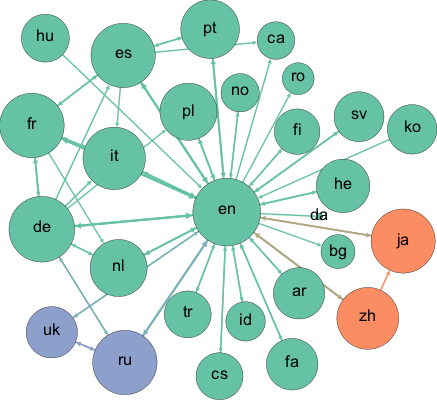
\includegraphics[scale=.5]{img/Wikipedia_multilingual_network_graph_July_2013.png}
	\caption{Wikipedia Multilingual Network Graph (July 2013)}
\end{figure}
\newpage
La relazione tra una coppia di nodi può essere di due tipi:
\begin{itemize}
	\item Simmetrica: l'arco connette i nodi con un collegamento bidirezionale ed è detto \textit{indiretto}. Un grafo costituito di soli archi indiretti è anch'esso detto indiretto.
	\item Asimmetrica: l'arco connette i nodi con un collegamento unidirezionale ed è detto \textit{diretto}. Un grafo costituito di soli archi diretti è anch'esso detto diretto.
\end{itemize}
\begin{figure}[h!]
	\vspace*{1cm}
	\begin{minipage}{0.45\textwidth}
	\centering
	\begin{tikzpicture}[-,>=stealth',shorten >=1pt,auto,node distance=2cm,
		thick,main node/.style={circle,draw,font=\sffamily\Large\bfseries}]
		\node[main node] (1) {1};
		\node[main node] (2) [below left of=1] {2};
		\node[main node] (3) [below right of=2] {3};
		\node[main node] (4) [below right of=1] {4};
		\path[every node/.style={font=\sffamily\small}]
		(1) edge node [left] {} (4)
		
		(2) edge node [right] {} (1)
		
		(3) edge node [right] {} (2)
		
		(4) edge node [left] {} (3);
		
	\end{tikzpicture}
	\caption{Grafo indiretto}
	\end{minipage}\hfill
% <-- needed to keep the imgs side by side
	\begin{minipage}{0.45\textwidth}
	\centering
	\begin{tikzpicture}[->,>=stealth',shorten >=1pt,auto,node distance=2cm,
		thick,main node/.style={circle,draw,font=\sffamily\Large\bfseries}]
		\node[main node] (1) {1};
		\node[main node] (2) [below left of=1] {2};
		\node[main node] (3) [below right of=2] {3};
		\node[main node] (4) [below right of=1] {4};
		\path[every node/.style={font=\sffamily\small}]
		(1) edge node [left] {} (4)
		
		(2) edge node [right] {} (1)
		
		(3) edge node [right] {} (2)
		
		(4) edge node [left] {} (3);
	\end{tikzpicture}
	\caption{Grafo diretto}
	\end{minipage}
\end{figure}
Un grafo può essere formalmente descritto come una coppia di insiemi \textbf{G = (V, E)}, dove V è l'insieme dei nodi ed E è l'insieme degli archi. Un arco e $\in$ E è rappresentato come un sottoinsieme di due elementi di V, $e = \lbrace u, v\rbrace$ per $u, v \in V$.\\
Le rappresentazioni atte a descrivere un grafo sono molteplici:
\begin{itemize}
	\item \textit{Rappresentazione grafica}: ad ogni nodo corrisponde una figura circolare sul piano e ad ogni arco (i, j) corrisponde una linea che che collega il nodo i al nodo j.
	\item \textit{Matrice di adiacenza}: matrice di dimensione $n \times n$, dove $n$ è il numero di nodi, il cui elemento (i, j) assume valore 1 se esiste l'arco tra il nodo i ed il nodo j, 0 altrimenti.
	\item \textit{Lista di adiacenza}: ad ogni vertice $v$ è associata la lista dei nodi ad esso vicini.
\end{itemize}
Negli anni, gli studi sulla teoria dei grafi hanno prodotto una quantità enorme di definizioni e teoremi, per cui, di seguito vengono descritti solamente i concetti necessari alla comprensione di questo lavoro di tesi.
\paragraph{Sottografo.} Un grafo H si dice sottografo di un grafo G se i vertici di H sono un sottoinsieme dei vertici di G e gli archi di H sono un sottoinsieme degli archi di G. Siano $G=(V, E)$ ed $H=(V_1, E_1)$ due grafi. H è un sottografo di G se e solo se $V_1 \subseteq V$ ed $E_1 \subseteq E$.
Un concetto particolarmente utile alla comprensione di questo lavoro è lo \textit{spanning subgraph}: uno spanning subgraph H di un grafo G è un sottografo che contiene tutti i vertici di G, cioé $V_1 = V$.
\paragraph{Grado di un nodo.} Il grado di un nodo $v$ è il numero di nodi ad esso adiacenti ed è indicato con \textit{deg(v)}.\\
In un grafo diretto, si distinguono due tipi di grado:
\begin{itemize}
	\item \textit{in-deg(v)}, il grado in ingresso del nodo \textit{v}, dato dal numero di archi in cui \textit{v} compare come nodo destinazione;
	\item \textit{out-deg(v)}, il grado in uscita del nodo \textit{v}, dato dal numero di archi in cui \textit{v} compare come nodo sorgente.
\end{itemize}
\paragraph{Cammino.} Un cammino è una sequenza di nodi, in cui ogni coppia consecutiva della sequenza sia connessa da un arco. Formalmente, un cammino è una sequenza di vertici $v_0, v_1, \cdots, v_n \in V$ tale che $\lbrace v_{i-1}, v_i\rbrace \in E, \forall 1\leq i \leq n$. Un cammino con almeno tre vertici distinti, i cui vertici di inizio e fine coincidono, è detto \textit{ciclo}.
\paragraph{Grafo connesso.} Un grafo è connesso se, per ogni coppia distinta di vertici (i, j), esiste un cammino da i a j.

\subsection{Grafo come modello della realtà}
I grafi hanno una grande utilità, in quanto consentono di astrarre le relazioni che intercorrono tra più oggetti, e di rappresentare tali relazioni in strutture su cui è possibile applicare modelli matematici. In \cite{easley2010networks} viene proposto un esempio reale: la Figura \ref{arpanet} rappresenta la struttura della rete Internet nel Dicembre del 1970, noto come ARPANET allora, composto solo da 13 macchine. I nodi rappresentano gli host, e vi è un arco tra due host se esiste una comunicazione diretta tra di essi.
\begin{figure}[h!]
	\centering
	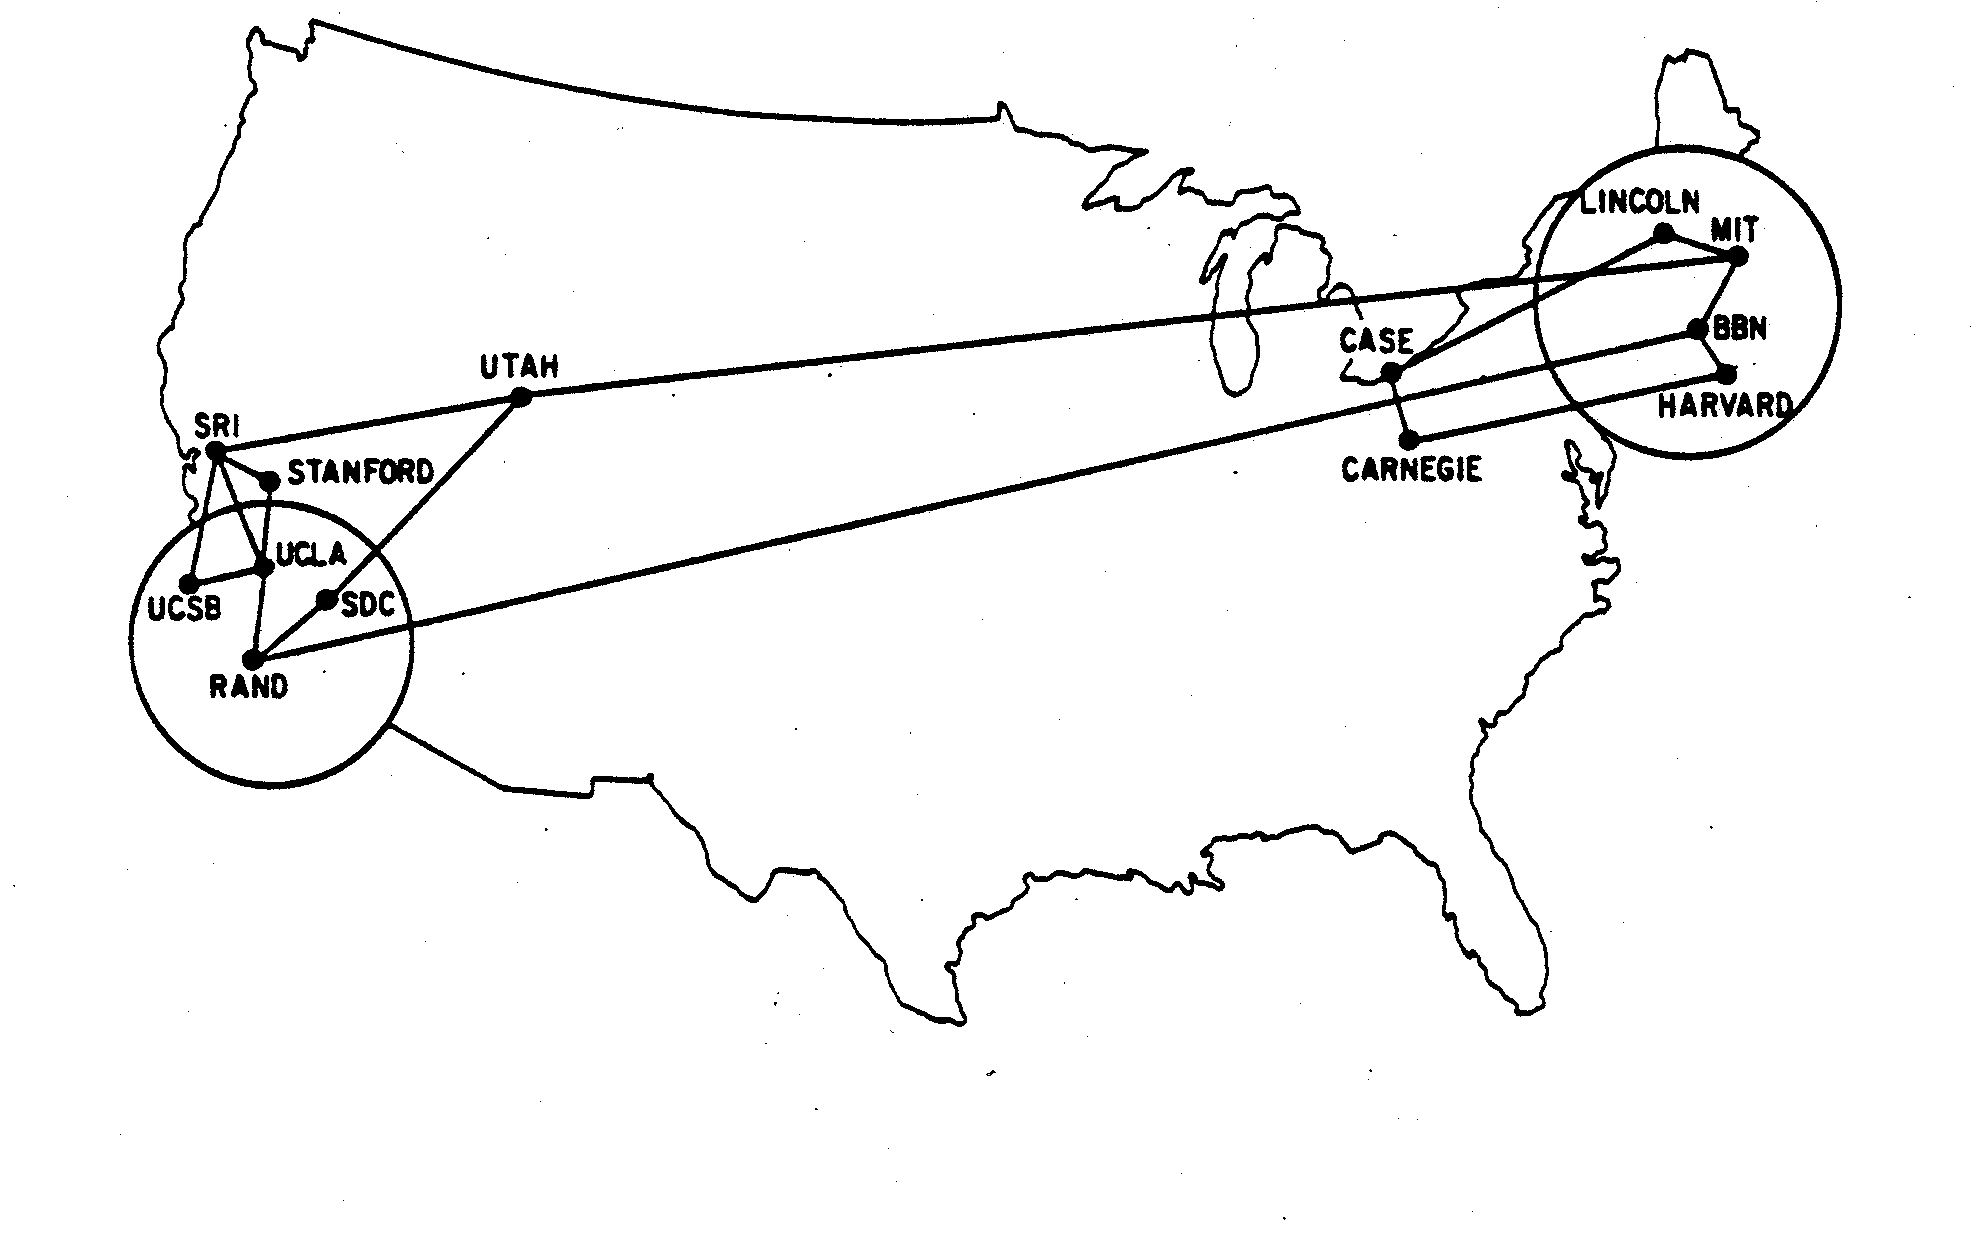
\includegraphics[scale=.7]{img/arpanetdec1970.jpg}
	\caption{ARPANET nel Dicembre 1970}
	\label{arpanet}
\end{figure}
Come è possibile intuire, la posizione geografica dei nodi non ha molta importanza, ma quel che conta è il come ogni nodo sia connesso agli altri. Infatti la figura \ref{arpanet_graph} mostra lo stesso grafo di ARPANET, attraverso una rappresentazione logica.
\begin{figure}
	\centering
	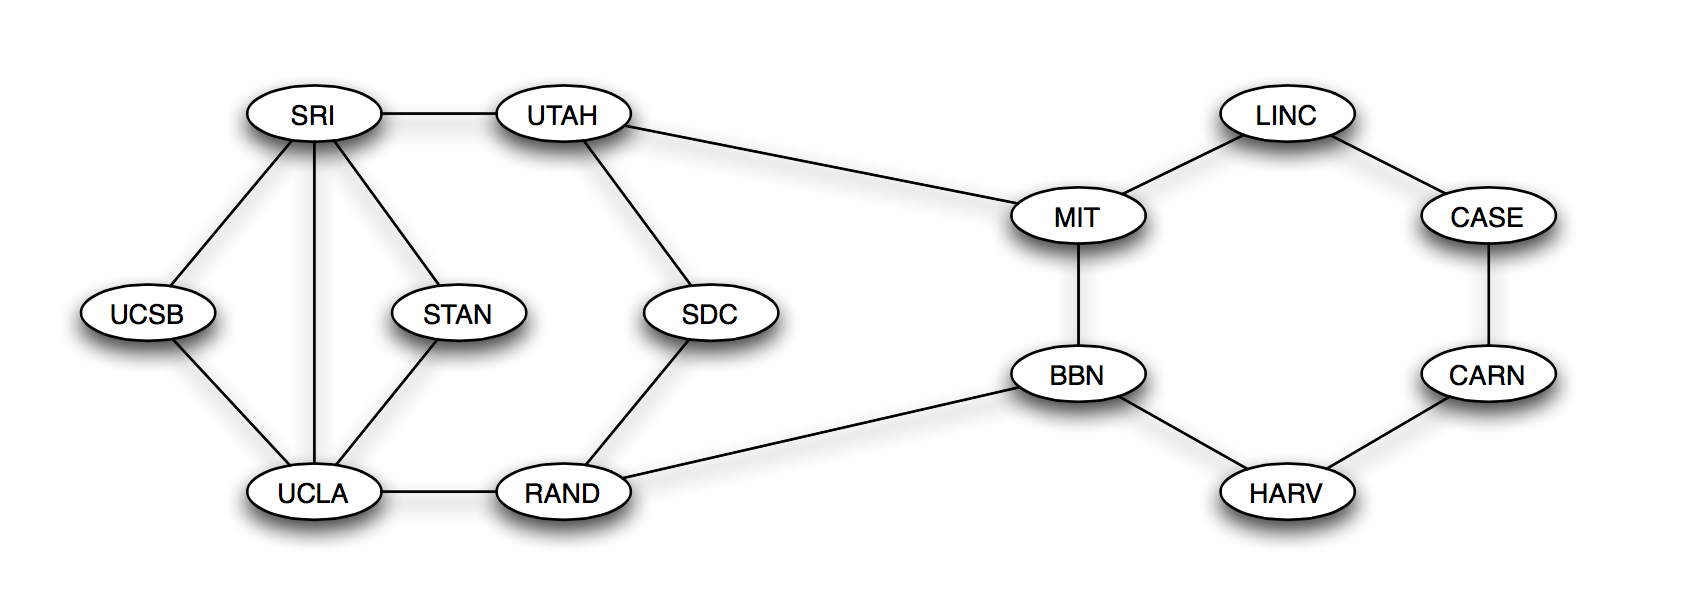
\includegraphics[scale=.5]{img/arpanetdec1970_graph.png}
	\caption{Grafo di ARPANET nel Dicembre 1970}
	\label{arpanet_graph}
\end{figure}
Il grafo di ARPANET mostrato in precedenza è un esempio di \textit{\textbf{communication network}}, i cui nodi sono computer o altri dispositivi capaci di inviare messaggi mentre gli archi rappresentano i collegamenti diretti lungo i quali tali messaggi possono viaggiare. Ma questo è solamente uno dei tipi di rete che possiamo avere.\\
Le \textit{\textbf{social network}} i cui nodi sono persone o gruppi di persone, ed i cui archi rappresentano un tipo di interazione (amicizia, inimicizia, ecc.), sono reti massive che al giorno d'oggi comprendono gran parte della popolazione mondiale, come ad esempio le reti di Facebook e Twitter.\\
Le \textit{\textbf{information network}} sono reti che rappresentano il mondo dell'informazione, i cui nodi sono le fonti di informazione e gli archi rappresentano collegamenti logici come riferimenti, citazioni identificati da hyperlink. A tale categoria appartiene il grafo del Web, così come la rete di documenti di Wikipedia.\\
Le \textit{\textbf{dependency network}}, che descrivono le dipendenze esistenti in una collezione di oggetti. Ne sono esempi reti di dipendenze tra task, per cui sono stati sviluppati molti lavori, applicati anche in altri campi come lo studio del sistema immunitario e delle reti semantiche.\\
I grafi mostrano la loro grande utilità anche nelle \textit{\textbf{transportation network}}, reti i cui nodi sono luoghi geografici ed i cui archi sono le linee stradali, ferroviarie o aeree che li collegano. Questo tipo di rete è stata di grande importanza nello sviluppo di concetti ed algoritmi su grafi, infatti molta della terminologia deriva dal mondo dei trasporti.\\
Quindi, come si evince dai vari tipi di network descritte finora, i grafi sono uno strumento potente che trova applicazione nelle realtà più disparate, partendo dalla matematica ed informatica, fino ad arrivare agli studi della sociologia, biologia, linguistica, chimica e fisica. Ed è proprio l'ultimo ambito ad interessare questo lavoro di tesi: la \textit{fisica statistica} è una branca della fisica che utilizza metodi della teoria delle probabilità e statistici, ed in particolare gli strumenti matematici usati per gestire grandi popolazioni ed approssimazioni, per la risoluzione di problemi fisici. Può descrivere una grande varietà di campi dotati di una natura stocastica intrinseca. Le sue applicazioni coinvolgono problemi nel campo della fisica, biologia, chimica, neurologia e scienze sociali.\\
Lo scopo finale per cui nasce la fisica statistica, in particolare la meccanica statistica, è quello di fornire strutture e strumenti per mettere in relazione proprietà microscopiche di atomi e molecole individuali rispetto a proprietà del materiale che possono essere osservate ad occhio nudo. Spiegando ad esempio la termodinamica come il risultato naturale di statistica, meccanica classica e meccanica quantistica al livello microscopico: il grafo riesce a modellare le particelle del sistema su cui agisce la dinamica del processo fisico.


\section{Modello di Ising}
Il modello di Ising è un classico problema combinatoriale della fisica statistica, studiato per la prima volta da Ernest Ising nel 1920. Tale modello è interessato alla fisica delle transizioni di fase, che occorrono quando un piccolo cambiamento nei parametri, come temperatura o pressione, causa un grande cambiamento qualitativo nello stato del sistema. Le transizioni di fase sono comuni nella fisica, come ad esempio nel fenomeno del ferromagnetismo.\\
Uno degli scopi principali del modello di Ising è spiegare come interazioni di breve raggio tra le componenti del sistema siano in grado di dare luogo a comportamenti correlati di lungo raggio e, quindi, di predire in un certo senso il potenziale per una transizione di fase. Tale modello trova applicazione in molti ambiti, in generale in tutti quegli ambiti dove si studia il comportamento cooperativo di grandi sistemi: tali applicazioni sono possibili perché il modello di Ising può essere formulato come un problema matematico. Una semplice definizione matematica del modello di Ising è data in \cite{cipra1987introduction} e in \cite{jerrum1993polynomial}: consideriamo una collezione di siti $\lbrack n \rbrack = \lbrace 0, 1, \cdots, n-1 \rbrace$, in cui ogni coppia $i, j$ ha associata un’energia di interazione $V_{ij}$. Nella maggior parte dei casi di interesse fisico, l’insieme E di coppie con energia di interazione non nulla forma un \textit{regular lattice graph} $([n], E)$: detto anche \textit{mesh graph} o \textit{grid graph}, è un grafo la cui rappresentazione grafica sul piano forma delle tassellature regolari.\\
Il primo passo del modello è quello di assegnare ad ogni sito \textit{i} una variabile $\sigma_i$, detta \textbf{spin}, con $i=1, \dots, n$. Le variabili $\sigma_i$ possono assumere solo due valori, $\sigma_i = \pm 1$, che si possono definire come gli \textit{stati} dei siti.\\
Una \textbf{configurazione} $\sigma$ del sistema è un assegnamento di spin positivi $\left( \sigma_i = 1 \right)$ o negativi $\left( \sigma_i = 1 \right)$ ad ogni sito $i \in \lbrack n \rbrack$.\\
L'\textit{energia} di una configurazione è data dall’Hamiltoniana del sistema: nella fisica matematica, tale quantità governa le dinamiche del sistema. Per il modello di Ising, l’Hamiltoniana è definita sotto un’assunzione ben precisa: si assume che solo le interazioni di breve raggio e con i siti più vicini e le interazioni dei siti con un ``campo esterno'' contribuiscono al livello di energia del sistema. Pertanto, per ogni configurazione $\sigma = (\sigma_1, \dots, \sigma_n)$ si ha:\\
\begin{equation}
H(\sigma) = - \sum_{\lbrace i,j \rbrace \in E}{V_{ij}\sigma_i\sigma_j} - B \sum_{k\in\lbrack n \rbrack}{\sigma_k}
\end{equation}

\subsection{Partition Function}

\section{Cenni di probabilità e statistica}

\section{Processi Markoviani}
\subsection{Irriducibilità e periodicità}
\subsection{Distribuzione stazionaria}
\subsection{Catena di Markov Monte Carlo}

\section{Algoritmi di approssimazione}